\chapter{Conservation de la masse et équations ajustées}\label{ch:g8:balanced-equations}

Une bûche de deux kilogrammes \omterm{def:g4:what-a-fire-needs:burning}{brûle} dans une cheminée. Au matin, il reste
quelques dizaines de grammes de cendre grise. Près de deux kilogrammes de
matière se sont-ils évanouis dans la nuit~? Pendant des siècles,
personne n'a su répondre. La réponse est venue d'un chimiste qui a
décidé de tout peser --- y compris les gaz, que personne n'avait songé
à peser.

\begin{recall}
Au cours d'une \omterm{def:g7:chemical-reactions:reaction}{réaction chimique}, les \omterm{def:g7:chemical-reactions:reactant}{réactifs} sont consommés et les
produits se forment~; les \omterm{def:g7:atoms-and-molecules:atom}{atomes} des \omterm{def:g7:chemical-reactions:reactant}{réactifs} se réarrangent pour former
les produits, sans être ni créés ni détruits
(\cref{ch:g7:chemical-reactions}). Une \omterm{def:g7:atoms-and-molecules:formula}{formule chimique} comme \ce{H2O}
énumère les \omterm{def:g7:atoms-and-molecules:atom}{atomes} d'une \omterm{def:g7:atoms-and-molecules:molecule}{molécule}~; un nombre placé devant, comme dans
\ce{3H2O}, compte des \omterm{def:g7:atoms-and-molecules:molecule}{molécules} (\cref{ch:g7:atoms-and-molecules}).
\end{recall}

\begin{omfigure}
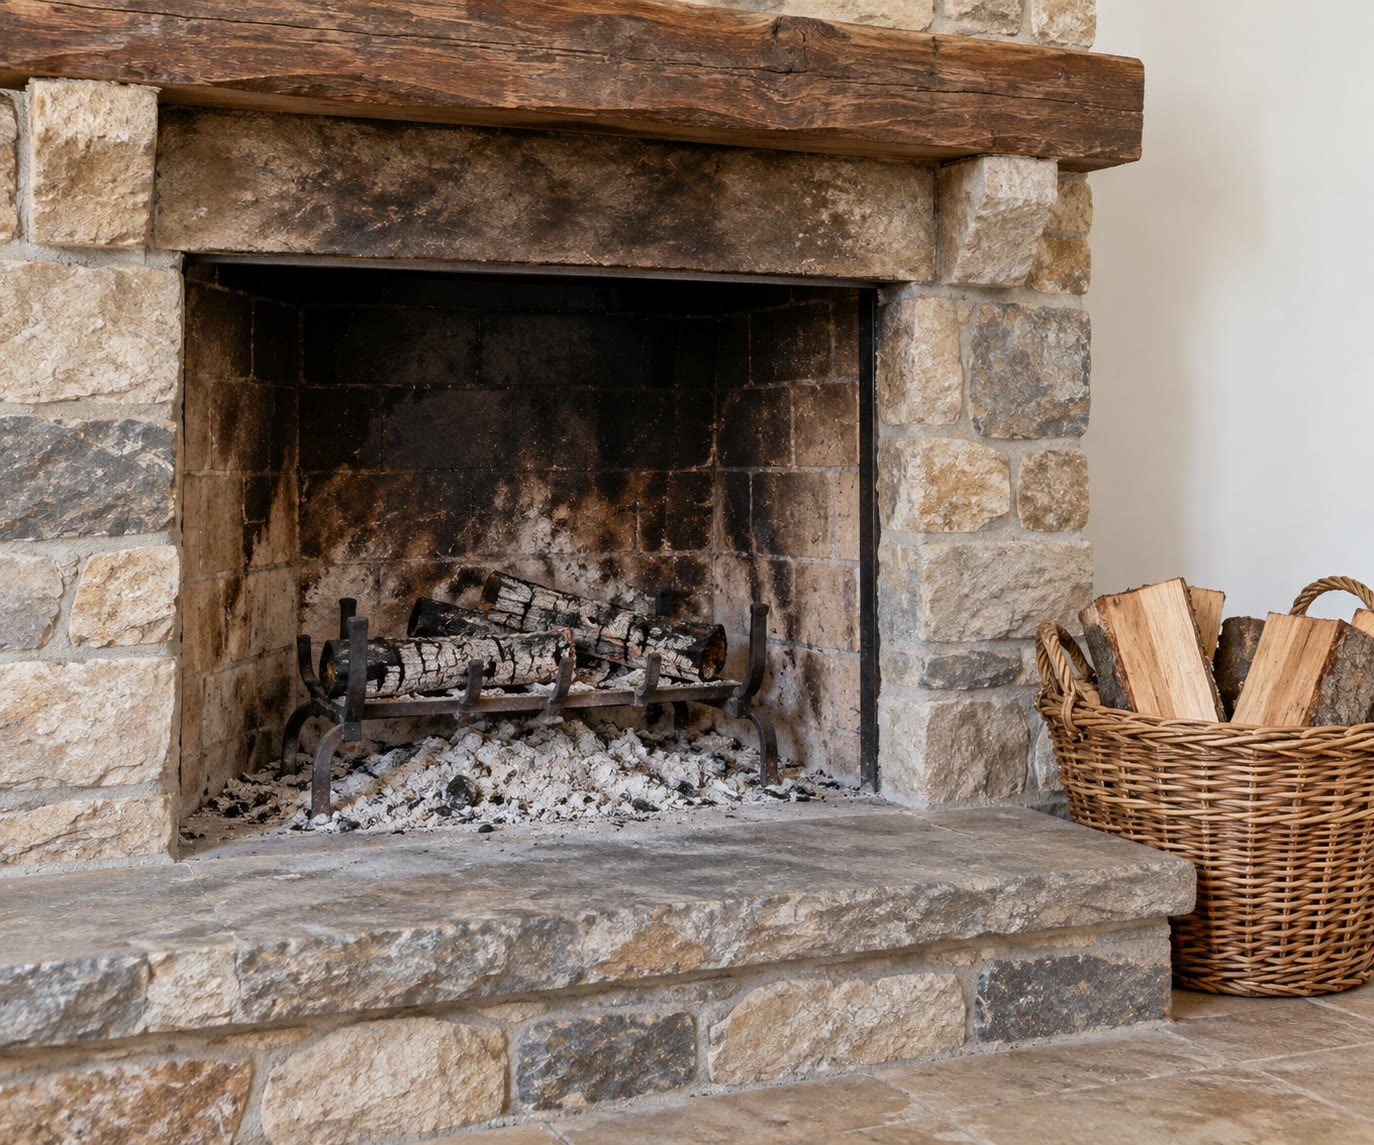
\includegraphics[width=0.5\linewidth]{images/book1/ai/g8-fireplace-ash.jpg}

{\small Une cheminée au petit matin~: un peu de cendre, c'est tout ce
qui reste des bûches.}
\end{omfigure}

\section{La masse se conserve}

\begin{inthelab}[Peser une réaction dans un flacon fermé]
L'enseignant verse un peu de vinaigre dans un erlenmeyer, met du
bicarbonate de soude dans un ballon de baudruche fixé sur son col, puis
pose le tout sur une balance~: \qty{212.4}{g}. On redresse le ballon
pour que le bicarbonate tombe dans le vinaigre~: le \omterm{def:g6:pure-substances-and-mixtures:mixture}{mélange} pétille et
le ballon se gonfle du gaz formé. La balance indique toujours
\qty{212.4}{g}. La même réaction dans un erlenmeyer ouvert, sans
ballon, «~perd~» de la masse~: le gaz s'échappe dans la pièce.
\end{inthelab}

\begin{omfigure}
\begin{tikzpicture}[font=\small, scale=1.15]
  % closed flask
  \pic[transform shape] at (0,0) {balance};
  \pic[transform shape] at (0,0.8) {erlenmeyer={0.25}{omWater!80}};
  \fill[red!55, draw=red!60!black] (0,4.05) ellipse (0.5 and 0.62);
  \fill[red!55] (-0.3,3.45) rectangle (0.3,3.6);
  \node[anchor=north, align=center] at (0,-0.1) {fermé~: le gaz reste\\ dans le ballon};
  \node[anchor=west, font=\footnotesize] at (1.25,0.3) {\qty{212.4}{g}};
  % open flask
  \pic[transform shape] at (4,0) {balance};
  \pic[transform shape] at (4,0.8) {erlenmeyer={0.25}{omWater!80}};
  \foreach \y in {3.6,3.95,4.3} \draw[->, black!45, decorate,
    decoration={snake, amplitude=0.6pt, segment length=4pt}] (4,\y) -- (4,\y+0.3);
  \node[anchor=north, align=center] at (4,-0.1) {ouvert~: le gaz s'échappe,\\ l'indication baisse};
  \node[anchor=west, font=\footnotesize] at (5.25,0.3) {\qty{211.9}{g}};
\end{tikzpicture}

{\small La même réaction, pesée. Dans l'erlenmeyer fermé, la masse ne
change pas~; dans l'erlenmeyer ouvert, le gaz s'en va et la balance
indique moins.}
\end{omfigure}

\begin{definition}[Conservation de la masse]\label{def:g8:balanced-equations:conservation}
La \emph{conservation de la masse}\index{conservation de la masse} est
la loi selon laquelle, au cours d'une \omterm{def:g7:chemical-reactions:reaction}{réaction chimique}, la masse totale
des produits formés est égale à la masse totale des \omterm{def:g7:chemical-reactions:reactant}{réactifs} consommés.
Rien ne se perd et rien ne se crée~; la matière ne fait que changer de
forme.
\end{definition}

\begin{example}[La bûche, pesée correctement]\label{ex:g8:balanced-equations:log}
Si l'on pouvait peser avant la bûche et le dioxygène qu'elle a pris à
l'\omterm{def:g4:air-a-mixture-of-gases:air}{air}, et après la cendre, le dioxyde de carbone et la vapeur d'eau, les
deux totaux seraient égaux. La cendre est légère parce que la plupart
des produits sont des gaz qui s'en vont par la cheminée.
\end{example}

\begin{history}[Lavoisier pèse tout, des années 1770 à 1789]
Antoine-Laurent Lavoisier s'imposa de peser chaque substance avant et
après chaque réaction, dans des récipients scellés, pour qu'aucun gaz ne
puisse s'échapper ni entrer. Il montra que les métaux gagnent de la masse
quand ils rouillent ou brûlent, en prenant quelque chose à l'\omterm{def:g4:air-a-mixture-of-gases:air}{air} --- le
dioxygène, auquel il donna le nom d'oxygène --- et affirma en 1789 que
rien ne se crée et rien ne se perd au cours d'une réaction. Sa femme,
Marie-Anne Paulze Lavoisier, travaillait à ses côtés, consignait les
expériences et dessina les appareils pour son livre.
\end{history}

\begin{omfigure}
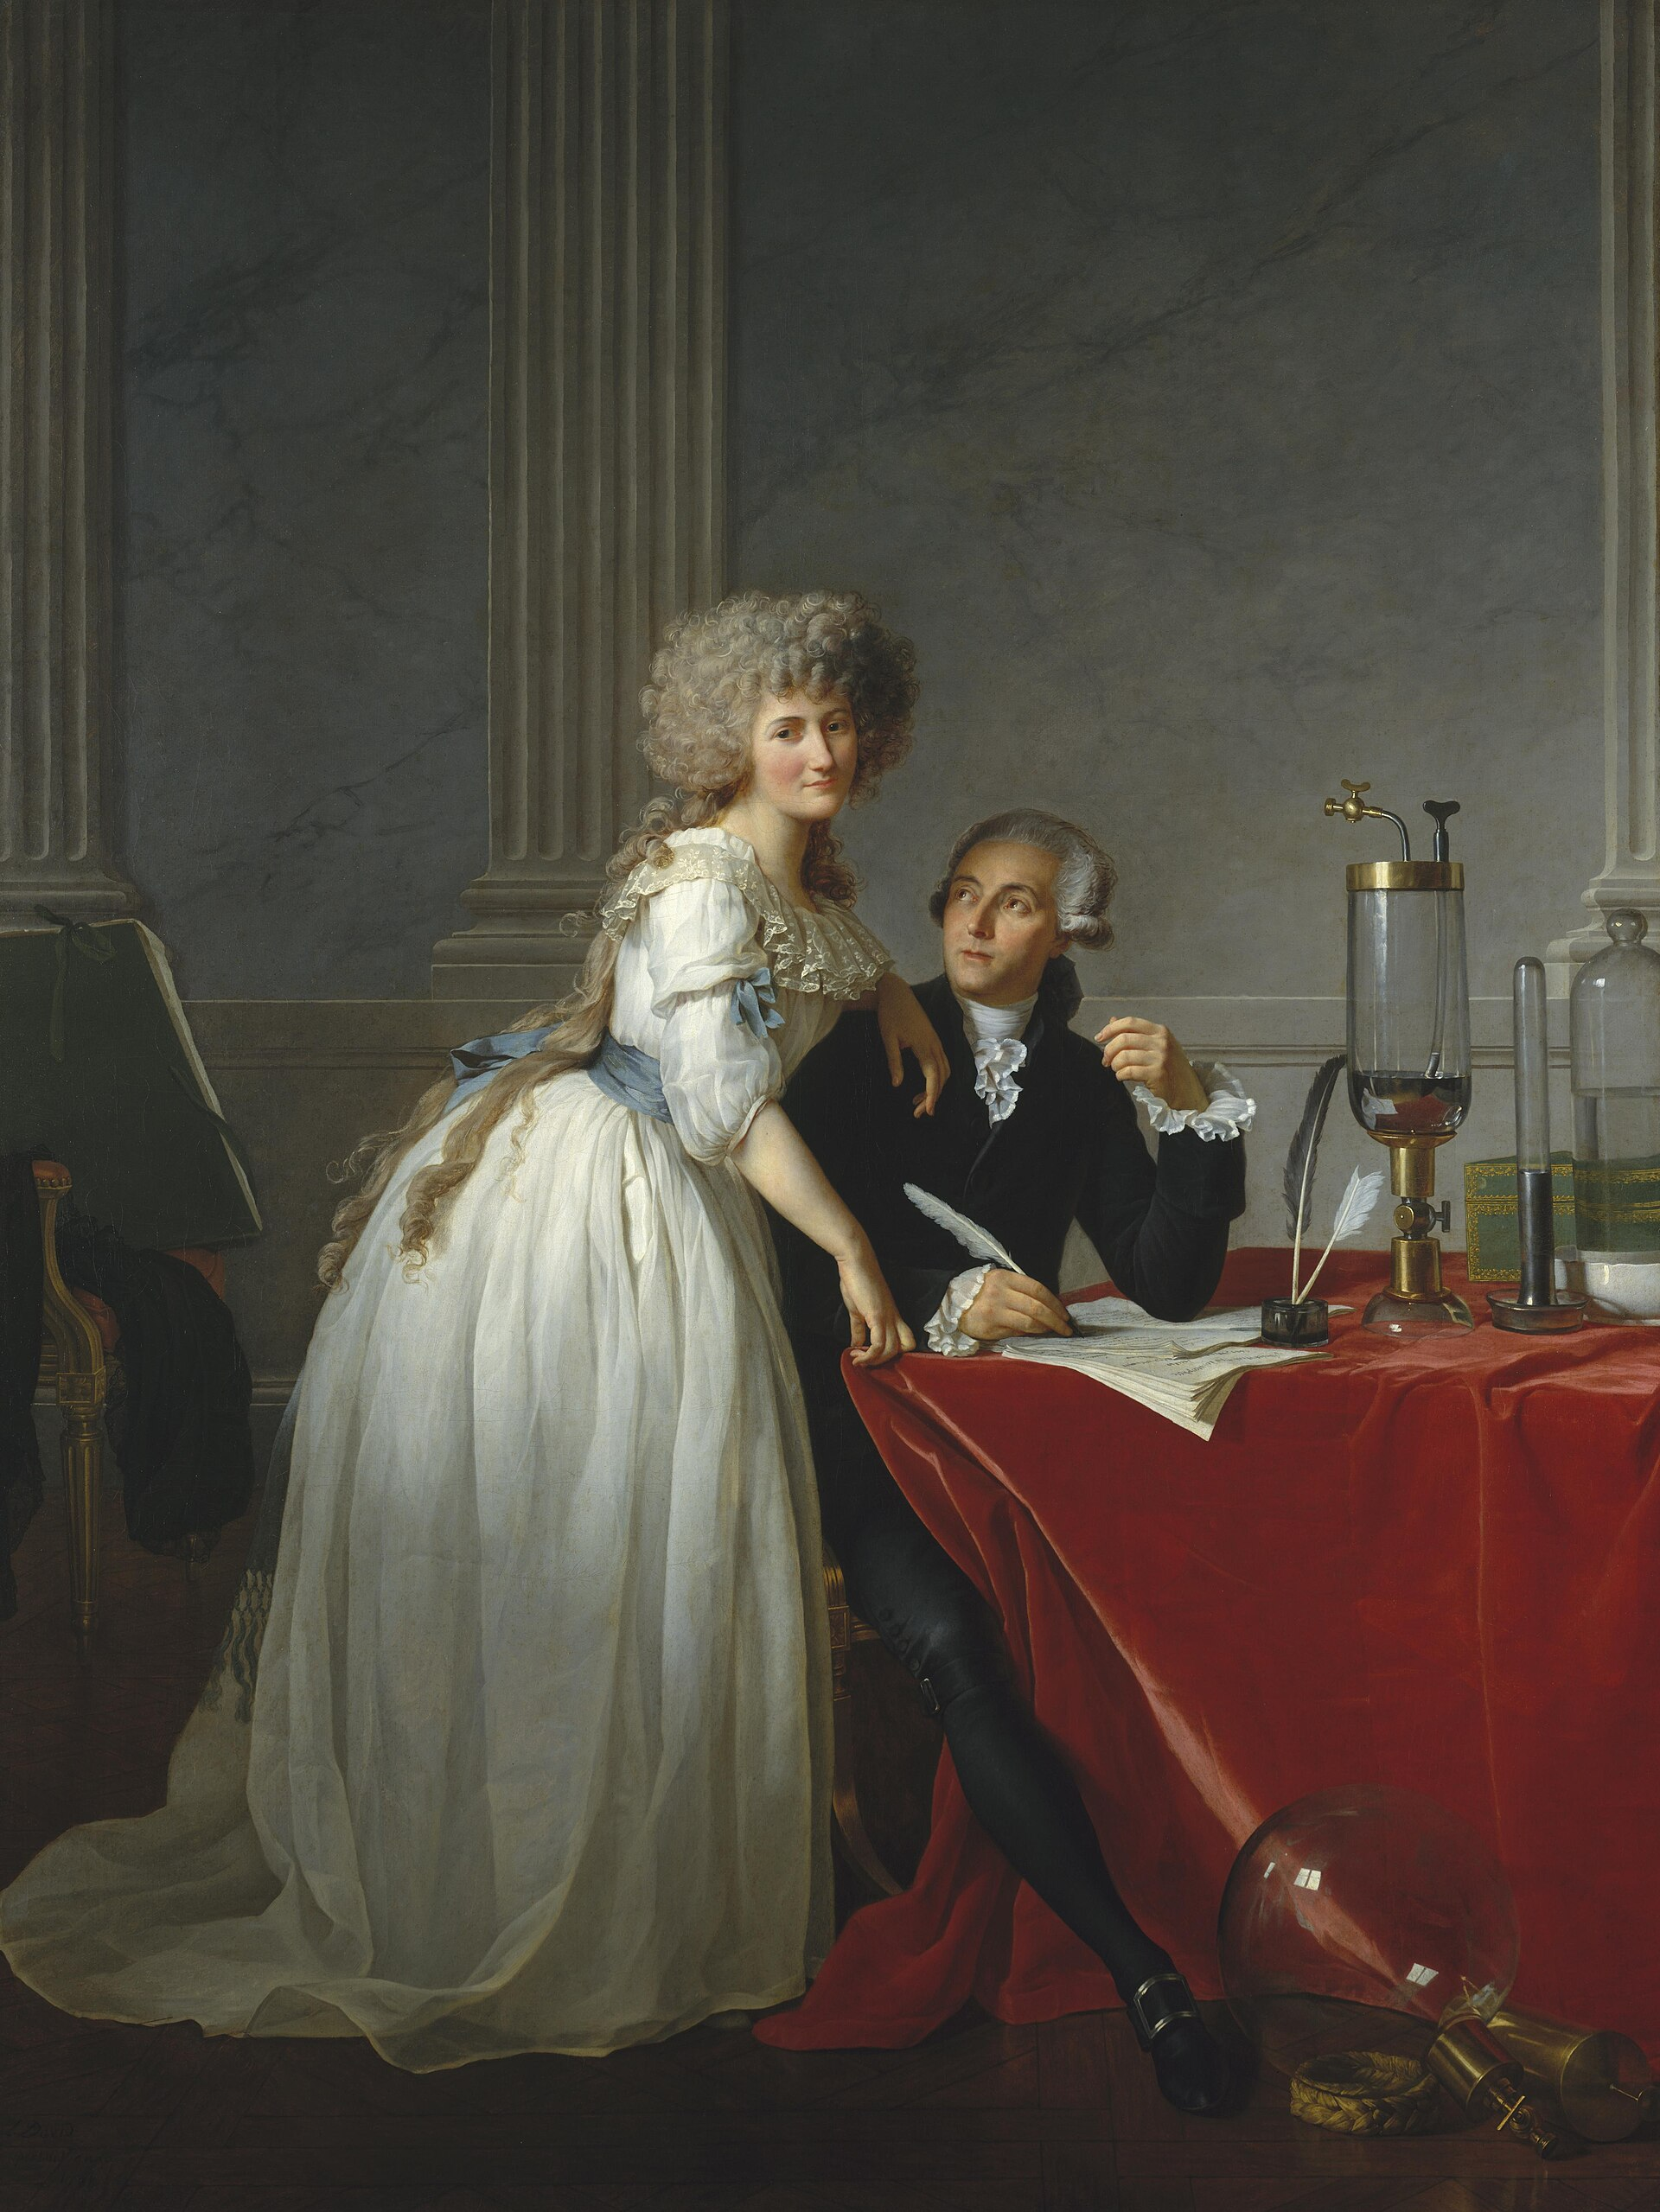
\includegraphics[width=0.3\linewidth]{images/book1/lavoisier.jpg}

{\small Antoine-Laurent Lavoisier et Marie-Anne Paulze Lavoisier, par
Jacques-Louis David, 1788.}
\end{omfigure}

\section{Pourquoi la masse se conserve}

\begin{proposition}[Les atomes se conservent, donc la masse se conserve]\label{prop:g8:balanced-equations:why}
Au cours d'une réaction, les \omterm{def:g7:atoms-and-molecules:atom}{atomes} sont seulement réarrangés~: chaque
\omterm{def:g7:atoms-and-molecules:atom}{atome} des \omterm{def:g7:chemical-reactions:reactant}{réactifs} se retrouve dans les produits. Chaque \omterm{def:g7:atoms-and-molecules:atom}{atome} garde sa
propre masse. La masse totale ne peut donc pas changer.
\end{proposition}

\begin{example}[Du fer qui prend de la masse]\label{ex:g8:balanced-equations:iron}
De la laine d'acier brûlée dans une coupelle ouverte posée sur une
balance devient plus lourde~: les \omterm{def:g7:atoms-and-molecules:atom}{atomes} de fer se sont liés à des \omterm{def:g7:atoms-and-molecules:atom}{atomes}
d'oxygène pris à l'\omterm{def:g4:air-a-mixture-of-gases:air}{air}, et l'oxyde de fer formé pèse autant que le fer
plus cet oxygène. Si on la \omterm{def:g4:what-a-fire-needs:burning}{brûle} dans un bocal d'\omterm{def:g4:air-a-mixture-of-gases:air}{air} scellé posé sur
la balance, l'ensemble ne change pas de masse~: le dioxygène était déjà
dans le bocal.
\end{example}

\section{L'équation chimique}

\begin{definition}[Équation chimique]\label{def:g8:balanced-equations:equation}
Une \emph{équation chimique}\index{equation chimique@équation chimique} écrit une réaction
avec des formules~: les formules des \omterm{def:g7:chemical-reactions:reactant}{réactifs} à gauche, reliées par
$+$, une flèche, et les formules des produits à droite. Chaque formule
peut être précédée d'un nombre. L'équation est une
\emph{équation ajustée}\index{equation ajustee@équation ajustée} quand chaque sorte
d'\omterm{def:g7:atoms-and-molecules:atom}{atome} apparaît le même nombre de fois des deux côtés.
\end{definition}

\begin{definition}[Coefficient stœchiométrique]\label{def:g8:balanced-equations:coefficient}
Le nombre écrit devant une formule dans une équation est son
\emph{coefficient stœchiométrique}\index{coefficient stoechiometrique@coefficient stœchiométrique}~:
il compte les \omterm{def:g7:atoms-and-molecules:molecule}{molécules} (ou les autres particules) de cette espèce qui
interviennent. Un coefficient 1 ne s'écrit pas.
\end{definition}

\begin{notation}[Symboles d'état]\label{not:g8:balanced-equations:states}
Une lettre entre parenthèses après une formule peut indiquer son état
physique~: (s) solide, (l) liquide, (g) gaz. Ainsi, \ce{H2O(l)} est de
l'eau liquide et \ce{H2O(g)} de la vapeur d'eau.
\end{notation}

\begin{example}[Lire une équation]\label{ex:g8:balanced-equations:read}
\[
  \ce{CH4(g) + 2O2(g) -> CO2(g) + 2H2O(l)}
\]
se lit~: une \omterm{def:g7:atoms-and-molecules:molecule}{molécule} de méthane et deux \omterm{def:g7:atoms-and-molecules:molecule}{molécules} de dioxygène
réagissent pour donner une \omterm{def:g7:atoms-and-molecules:molecule}{molécule} de dioxyde de carbone et deux
\omterm{def:g7:atoms-and-molecules:molecule}{molécules} d'eau. À gauche~: 1 C, 4 H, 4 O. À droite~: 1 C, 4 H,
$2 + 2 = 4$ O. L'équation est ajustée.
\end{example}

\begin{omfigure}
\begin{tikzpicture}[font=\small]
  \begin{scope}[every node/.style={font=\Large, inner sep=2pt}]
    \node (a) at (0,0) {\ce{CH4}};
    \node (p1) at (0.95,0) {$+$};
    \node (b) at (1.9,0) {\ce{2O2}};
    \node (arr) at (3.35,0) {$\longrightarrow$};
    \node (c) at (4.8,0) {\ce{CO2}};
    \node (p2) at (5.75,0) {$+$};
    \node (d) at (6.8,0) {\ce{2H2O}};
  \end{scope}
  \draw[thick, omDef] ([yshift=-2pt]a.south west) -- ++(0,-0.15) -| ([yshift=-2pt]b.south east);
  \node[below=8pt, text=black] at ($(a.south)!0.5!(b.south)$) {réactifs};
  \draw[thick, omProp] ([yshift=-2pt]c.south west) -- ++(0,-0.15) -| ([yshift=-2pt]d.south east);
  \node[below=8pt, text=black] at ($(c.south)!0.5!(d.south)$) {produits};
  \node[above=6pt of arr, font=\small] {«~réagissent pour donner~»};
  \node[anchor=north west, align=left, draw=black!35, rounded corners=2pt,
    font=\small, inner sep=4pt] at (-0.3,-1.25)
    {Dans \ce{2O2}~: le grand 2 devant est le \textbf{coefficient} (deux molécules)~;\\
     le petit 2 en bas à droite est l'\textbf{indice} (deux atomes dans chaque molécule).};
\end{tikzpicture}

{\small Les parties d'une \omterm{def:g8:balanced-equations:equation}{équation chimique}.}
\end{omfigure}

\section{Ajuster une équation}

\begin{method}[Ajuster une équation]\label{met:g8:balanced-equations:balance}
\begin{enumerate}
  \item Écrire les formules correctes des \omterm{def:g7:chemical-reactions:reactant}{réactifs} et des produits. Ne
        jamais modifier une formule ensuite~: changer \ce{H2O} en
        \ce{H2O2} décrirait une autre substance.
  \item Compter les \omterm{def:g7:atoms-and-molecules:atom}{atomes} de chaque sorte de chaque côté.
  \item Ajuster une sorte d'\omterm{def:g7:atoms-and-molecules:atom}{atome} à la fois avec des coefficients, en
        commençant par les \omterm{def:g7:atoms-and-molecules:atom}{atomes} qui n'apparaissent que dans une seule
        formule de chaque côté~; garder l'hydrogène et l'oxygène pour la
        fin.
  \item Compter de nouveau~; recommencer jusqu'à ce que chaque sorte
        d'\omterm{def:g7:atoms-and-molecules:atom}{atome} soit ajustée.
  \item Utiliser les plus petits nombres entiers.
\end{enumerate}
\end{method}

\begin{example}[Dihydrogène et dioxygène]\label{ex:g8:balanced-equations:water}
Non ajustée~: \ce{H2 + O2 -> H2O} % ce-unbalanced-ok (the skeleton)
a 2 O à gauche, 1 à droite. On place 2 devant \ce{H2O}~: il y a
maintenant 4 H à droite, donc on place 2 devant \ce{H2}~:
\[
  \ce{2H2 + O2 -> 2H2O}.
\]
Vérification~: 4 H et 2 O de chaque côté.
\end{example}

\begin{example}[Le fer qui brûle dans le dioxygène]\label{ex:g8:balanced-equations:iron-oxide}
Le fer et le dioxygène donnent l'oxyde de fer \ce{Fe2O3}. Oxygène~: 2 à
gauche, 3 à droite~; le plus petit nombre commun est 6, donc 3 \ce{O2}
et 2 \ce{Fe2O3}. Il y a alors 4 Fe à droite, donc 4 Fe à gauche~:
\[
  \ce{4Fe + 3O2 -> 2Fe2O3}.
\]
\end{example}

\begin{omfigure}
\begin{tikzpicture}[font=\small]
  % 2 H2
  \foreach \y in {0.45,-0.45} {
    \node[aH] (a) at (0,\y) {}; \node[aH] (b) at (0.45,\y) {};
    \begin{scope}[on background layer]\draw[bond] (a.center) -- (b.center);\end{scope}}
  \node at (1.05,0) {$+$};
  \node[aO] (a) at (1.6,0) {}; \node[aO] (b) at (2.25,0) {};
  \begin{scope}[on background layer]
    \draw[bond, line width=1.1pt] ([yshift=1.6pt]a.center) -- ([yshift=1.6pt]b.center);
    \draw[bond, line width=1.1pt] ([yshift=-1.6pt]a.center) -- ([yshift=-1.6pt]b.center);
  \end{scope}
  \draw[->, thick, omProp] (2.9,0) -- (3.9,0);
  \foreach \y in {0.5,-0.5} {
    \node[aO] (o) at (4.9,\y+0.12) {};
    \node[aH] (p) at (4.35,\y-0.28) {}; \node[aH] (q) at (5.45,\y-0.28) {};
    \begin{scope}[on background layer]
      \draw[bond] (o.center) -- (p.center); \draw[bond] (o.center) -- (q.center);
    \end{scope}}
  \node[align=center, font=\footnotesize] at (1.1,-1.35) {4 H, 2 O};
  \node[align=center, font=\footnotesize] at (4.9,-1.35) {4 H, 2 O};
  \node[font=\small] at (2.7,-2.0) {\ce{2H2 + O2 -> 2H2O}};
\end{tikzpicture}

{\small L'\omterm{def:g8:balanced-equations:equation}{équation ajustée} de la \omterm{def:g4:what-a-fire-needs:burning}{combustion} du dihydrogène, dessinée
avec des modèles~: deux \omterm{def:g7:atoms-and-molecules:molecule}{molécules} de dihydrogène et une \omterm{def:g7:atoms-and-molecules:molecule}{molécule} de
dioxygène donnent deux \omterm{def:g7:atoms-and-molecules:molecule}{molécules} d'eau.}
\end{omfigure}

\section{Lire une équation en molécules}


\begin{proposition}[Ce que dit une équation ajustée]\label{prop:g8:balanced-equations:molecules}
Les coefficients d'une \omterm{def:g8:balanced-equations:equation}{équation ajustée} donnent les proportions dans
lesquelles les particules réagissent et se forment. Si l'équation est
\ce{2H2 + O2 -> 2H2O}, alors 200 \omterm{def:g7:atoms-and-molecules:molecule}{molécules} de dihydrogène réagissent avec
100 \omterm{def:g7:atoms-and-molecules:molecule}{molécules} de dioxygène pour donner 200 \omterm{def:g7:atoms-and-molecules:molecule}{molécules} d'eau~; un million
de \omterm{def:g7:atoms-and-molecules:molecule}{molécules} de dioxygène demandent deux millions de \omterm{def:g7:atoms-and-molecules:molecule}{molécules} de
dihydrogène.
\end{proposition}

\begin{example}[Le propane d'un réchaud de camping]\label{ex:g8:balanced-equations:propane}
Le propane, \ce{C3H8}, \omterm{def:g4:what-a-fire-needs:burning}{brûle} dans le dioxygène en donnant du dioxyde de
carbone et de l'eau. Le carbone d'abord~: 3 C, donc 3 \ce{CO2}.
L'hydrogène~: 8 H, donc 4 \ce{H2O}. L'oxygène à droite~:
$3 \times 2 + 4 = 10$ O, donc 5 \ce{O2}~:
\[
  \ce{C3H8 + 5O2 -> 3CO2 + 4H2O}.
\]
Chaque \omterm{def:g7:atoms-and-molecules:molecule}{molécule} de propane a besoin de cinq \omterm{def:g7:atoms-and-molecules:molecule}{molécules} de dioxygène.
\end{example}

\section{Exercices}

\begin{exercise}[$\star$]\label{exo:g8:balanced-equations:1}
Énonce la loi de \omterm{def:g8:balanced-equations:conservation}{conservation de la masse}.
\end{exercise}

\begin{exercise}[$\star$]\label{exo:g8:balanced-equations:2}
Dans \ce{3CO2}, quel est le \omterm{def:g8:balanced-equations:coefficient}{coefficient stœchiométrique}~? Combien
d'\omterm{def:g7:atoms-and-molecules:atom}{atomes} de carbone et combien d'\omterm{def:g7:atoms-and-molecules:atom}{atomes} d'oxygène cela représente-t-il~?
\end{exercise}

\begin{exercise}[$\star$]\label{exo:g8:balanced-equations:3}
L'équation \ce{C + O2 -> CO2} est-elle ajustée~? Compte les \omterm{def:g7:atoms-and-molecules:atom}{atomes} pour
le vérifier.
\end{exercise}

\begin{exercise}[$\star$]\label{exo:g8:balanced-equations:4}
Ajuste \ce{Mg + O2 -> MgO}. % ce-unbalanced-ok (to balance)
\end{exercise}

\begin{exercise}[$\star\star$]\label{exo:g8:balanced-equations:5}
Ajuste \ce{N2 + H2 -> NH3}, la réaction qui produit l'ammoniac. % ce-unbalanced-ok (to balance)
\end{exercise}

\begin{exercise}[$\star\star$]\label{exo:g8:balanced-equations:6}
\qty{12}{g} de carbone brûlent complètement et forment \qty{44}{g} de
dioxyde de carbone. Quelle masse de dioxygène a été consommée~?
\end{exercise}

\begin{exercise}[$\star\star$]\label{exo:g8:balanced-equations:7}
Regarde la figure des deux erlenmeyers sur des balances. Pourquoi
l'indication de l'erlenmeyer ouvert baisse-t-elle~? De la masse a-t-elle
été détruite~?
\end{exercise}

\begin{exercise}[$\star\star$]\label{exo:g8:balanced-equations:8}
Ajuste \ce{CH4 + O2 -> CO2 + H2O} pas à pas, en indiquant quel \omterm{def:g7:atoms-and-molecules:atom}{atome} tu % ce-unbalanced-ok (to balance)
ajustes à chaque étape.
\end{exercise}

\begin{exercise}[$\star\star$]\label{exo:g8:balanced-equations:9}
Un élève ajuste \ce{H2 + O2 -> H2O} en écrivant \ce{H2 + O2 -> H2O2}. % ce-unbalanced-ok (the student's start)
Pourquoi est-ce faux~?
\end{exercise}

\begin{exercise}[$\star\star$]\label{exo:g8:balanced-equations:10}
D'après \ce{C3H8 + 5O2 -> 3CO2 + 4H2O}, combien de \omterm{def:g7:atoms-and-molecules:molecule}{molécules} de
dioxygène faut-il pour \omterm{def:g4:what-a-fire-needs:burning}{brûler} 20 \omterm{def:g7:atoms-and-molecules:molecule}{molécules} de propane~? Combien de
\omterm{def:g7:atoms-and-molecules:molecule}{molécules} d'eau se forment~?
\end{exercise}

\begin{exercise}[$\star\star\star$]\label{exo:g8:balanced-equations:11}
Ajuste \ce{C2H6 + O2 -> CO2 + H2O}, la \omterm{def:g4:what-a-fire-needs:burning}{combustion} de l'éthane. (Indice~: % ce-unbalanced-ok (to balance)
essaie de doubler l'éthane.)
\end{exercise}

\begin{exercise}[$\star\star\star$]\label{exo:g8:balanced-equations:12}
Une bougie de \qty{20.0}{g} \omterm{def:g4:what-a-fire-needs:burning}{brûle} dans une boîte en verre scellée,
pleine d'\omterm{def:g4:air-a-mixture-of-gases:air}{air}, posée sur une balance qui indique \qty{850.0}{g} en tout.
Quand la flamme s'éteint, la bougie pèse \qty{19.6}{g}. Qu'indique la
balance~? Explique.
\end{exercise}

\section{Problème~: de la laine d'acier dans un bocal scellé}

\begin{problem}[{Problème du week-end --- du fer qui brûle, une balance
qui ne bouge pas, et le dioxygène pris à l'air}]
\label{pb:g8:balanced-equations:1}
Au laboratoire, un enseignant \omterm{def:g4:what-a-fire-needs:burning}{brûle} de la laine d'acier, qui est du fer
presque pur, de deux façons. D'abord, un tampon est brûlé dans une
coupelle ouverte posée sur une balance~: l'indication augmente. Puis un
tampon de \qty{0.28}{g} est brûlé, enflammé par une étincelle électrique,
à l'intérieur d'un bocal d'\omterm{def:g4:air-a-mixture-of-gases:air}{air} fermé posé sur la balance~: l'indication
ne change pas. Le bocal contient environ \qty{0.5}{g} de dioxygène. Le
fer qui \omterm{def:g4:what-a-fire-needs:burning}{brûle} dans le dioxygène forme l'oxyde de fer \ce{Fe2O3}~; avec
moins de dioxygène, il peut aussi former \ce{Fe3O4}.

\medskip
\noindent\textbf{Partie I --- Deux pesées.}
\begin{enumerate}
  \item Dans la coupelle ouverte, la masse augmente. D'où vient la masse
        supplémentaire~?
  \item Dans le bocal fermé, la masse ne change pas. Explique.
  \item Énonce la loi illustrée par ces deux pesées.
\end{enumerate}

\medskip
\noindent\textbf{Partie II --- Deux équations.}
\begin{enumerate}[resume]
  \item Ajuste l'équation \ce{Fe + O2 -> Fe2O3}. % ce-unbalanced-ok (to balance)
  \item Ajuste l'équation \ce{Fe + O2 -> Fe3O4}. % ce-unbalanced-ok (to balance)
  \item Vérifie la première équation en comptant les \omterm{def:g7:atoms-and-molecules:atom}{atomes} de chaque
        sorte de chaque côté.
  \item D'après la première équation, combien de \omterm{def:g7:atoms-and-molecules:molecule}{molécules} de dioxygène
        réagissent avec 400 \omterm{def:g7:atoms-and-molecules:atom}{atomes} de fer~?
\end{enumerate}

\medskip
\noindent\textbf{Partie III --- Les masses.}
Dans \ce{Fe2O3}, chaque \qty{7}{g} de fer est combiné à \qty{3}{g}
d'oxygène. Le tampon de \qty{0.28}{g} \omterm{def:g4:what-a-fire-needs:burning}{brûle} entièrement en \ce{Fe2O3}.
\begin{enumerate}[resume]
  \item Quelle masse d'oxygène se combine à \qty{0.28}{g} de fer~?
  \item Quelle est la masse d'oxyde de fer formée~?
  \item Y avait-il assez de dioxygène dans le bocal~? Explique.
  \item On ouvre le bocal après refroidissement, et l'\omterm{def:g4:air-a-mixture-of-gases:air}{air} s'y engouffre.
        Explique pourquoi, et dis comment l'indication de la balance
        change alors.
  \item Calcule la masse de dioxygène prise à l'\omterm{def:g4:air-a-mixture-of-gases:air}{air} du bocal par la laine
        d'acier qui a brûlé.
\end{enumerate}
\end{problem}
